%%%%%%%%%%%%%%%%%%%%%%%%%%%%%%%%%%%%%%%%%%%%%%%%%%%%%%%%%%%%%%%%%%

\chapter{Conceptual Model/Model Geometry}
\label{Chap-ConcMod}

Introduction:

Basing on the descriptions of the preceding Chapter \ref{Chap-SouMas}, the water balance of the Chtouka aquifer can be regarded as shown in Figure \ref{Fig-SchemeBalance}: First of, groundwater directly enters and leaves the volume of the aquifer at its boundaries. 
Additional recharge is naturally provided by local rainfalls and infiltration from the Massa River, as well as from the YBT reservoir. 
At the same time, the Massa River can act as a drain of the aquifer, depending on its current gauge. 
Artificially, water is withdrawn for drinking and irrigation. 
As the irrigation water is applied to the irrigation perimeters at the surface of the aquifer, a partition of the irrigation water reinfiltrates into the aquifer. 
The other part however is lost due to evapotranspiration.

In this chapter the conceptual model following from this schematic water balance is described. 
Therefore, the aquifer is first delineated and its boundaries are characterised (Section \ref{Sec-Delineation}). 
Then the geological model of the aquifer volume is described, as it was derived by \textcite{Horn.2021} (Section \ref{Sec-GeolModel}). 
In the subsequent Sections \ref{Sec-PrecRech}-\ref{Sec-IrrRech} the other sources and sinks of the water balance are specified. 
At last, in Section \ref{Sec-Piezometers} the piezometers, which represent the observation points of the model are described.

\begin{figure}[h]
    \centering
    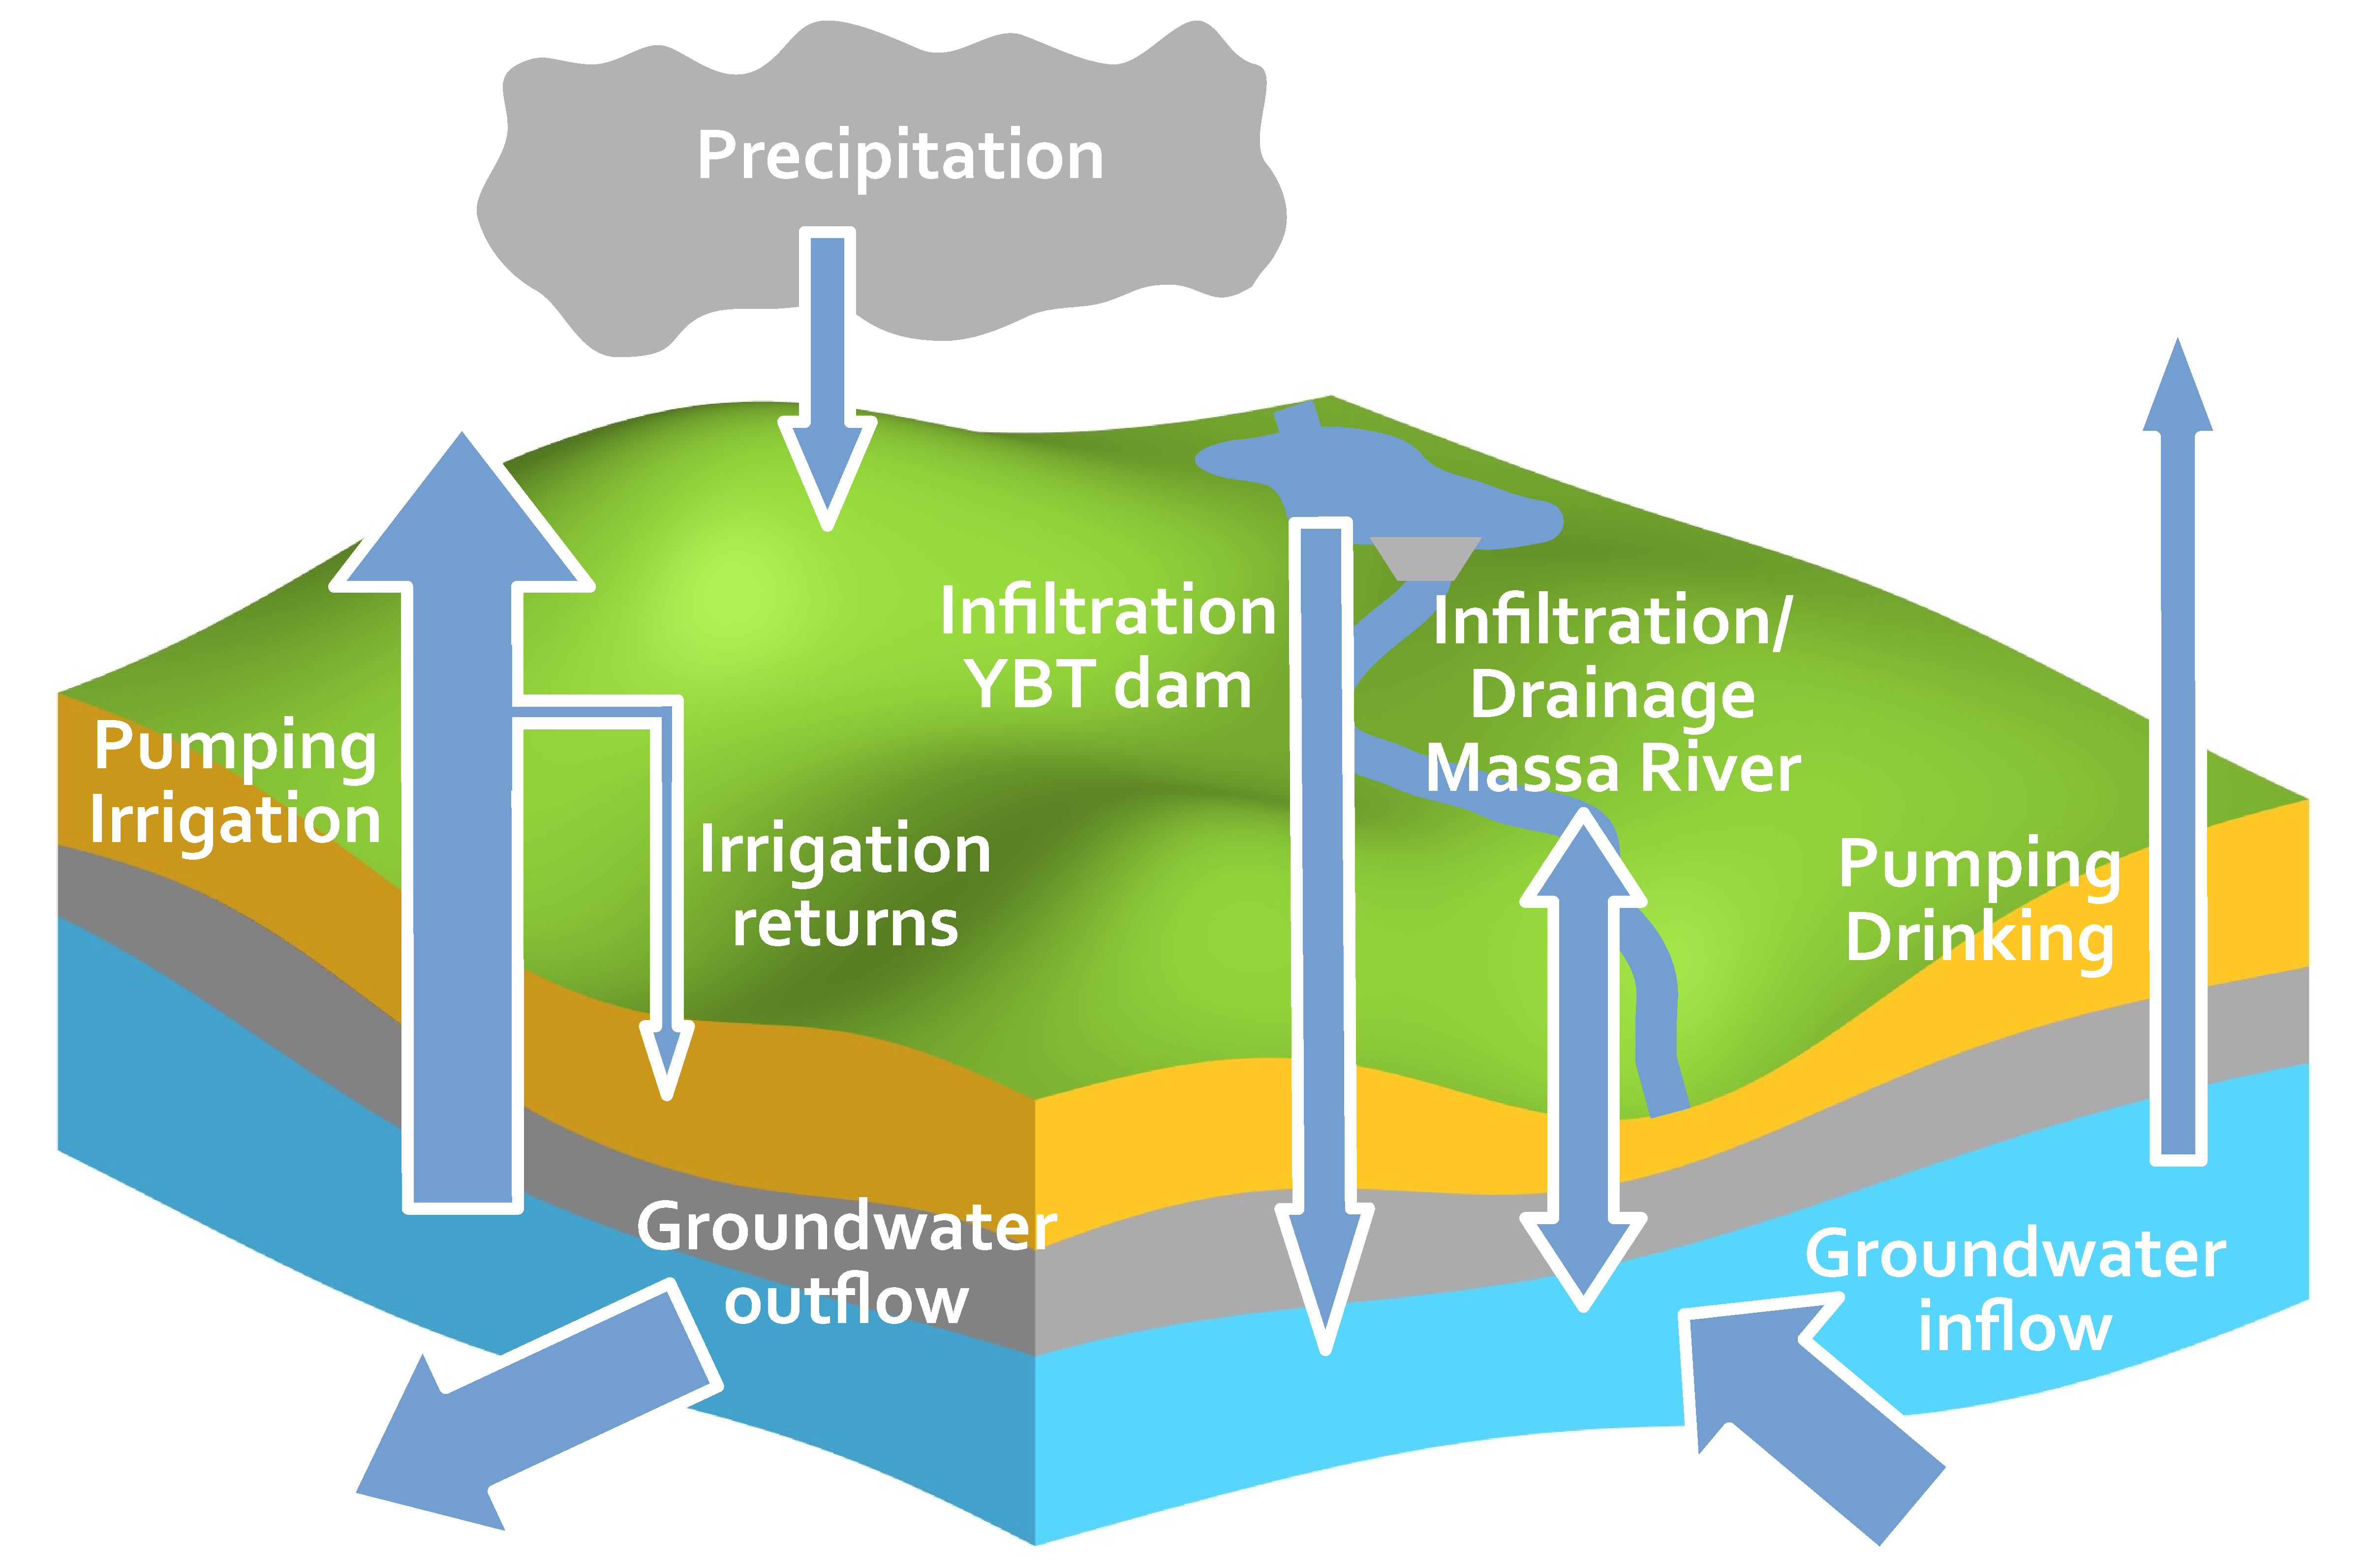
\includegraphics[width=1.0\textwidth]{./img/Fig-SchematicBalanceSystem.pdf}
    \caption{The water balance of the system.}
    \label{Fig-SchemeBalance}
\end{figure}

%%%%%%%%%%%%%%%%%%%%%%%%%%%%%%%%%%%%%%%%%%%%%%%%%%%%%%%%%%%%%%%%%%

\section{Delineation of the Model}
\label{Sec-Delineation}

For delineation in the $xy$-plane, a set of four boundaries, each characterised by a particular type of boundary condition has been characterised by \cite{Horn.2021}. 
These different boundaries approximately follow the orientation of the model outline in space and are therefore named as \textit{northern, eastern, southern} and \textit{western boundary}. 
The four boundaries are shown in Figure \ref{Map-BCPzPrec}. 
Their exact course is defined by \textcite{Anzar.2016}.

\begin{figure}[h]
    \centering
    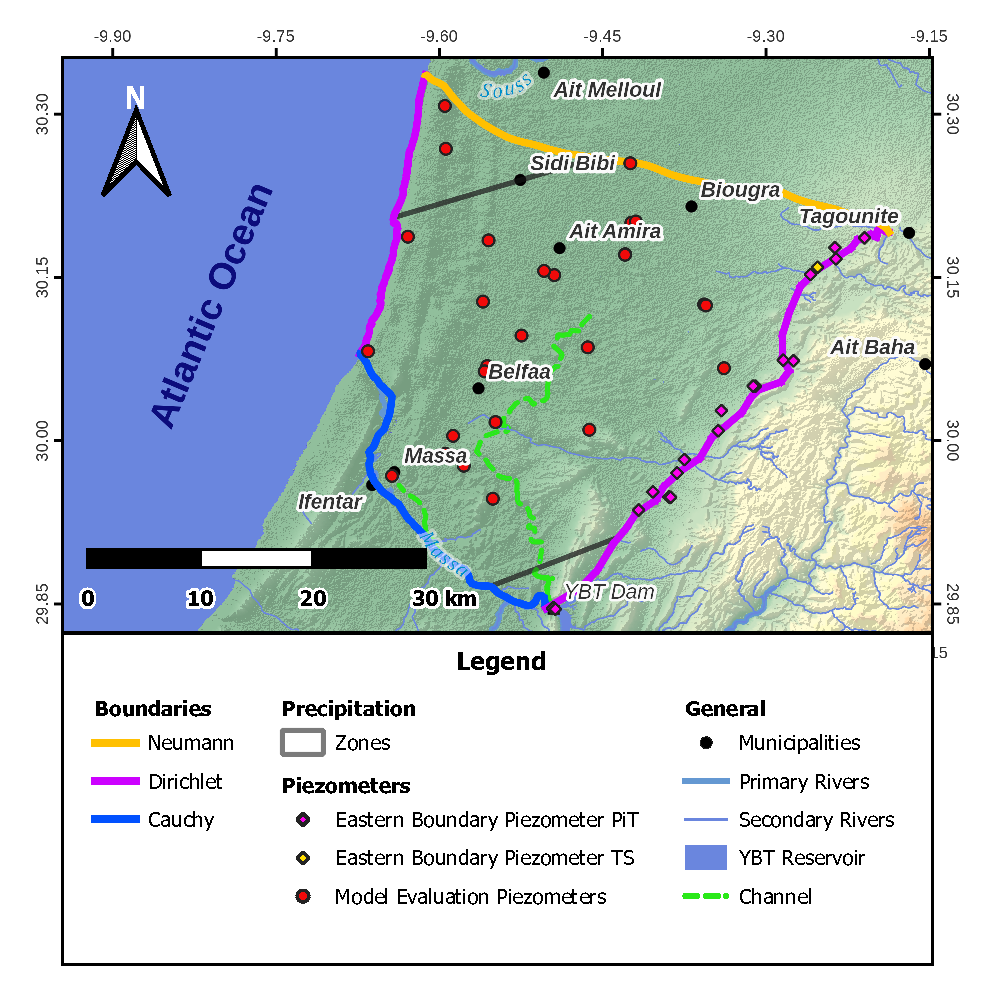
\includegraphics{./img/Map-BCPzPrec.pdf}
    \caption{Main components of the Chtouka aquifer conceptual model. For clarity, only the boundaries seperating the three precipitation areas are depicted. For the piezometers used to define the eastern boundary condition, PiT means point-in-time measurements and TS time series.}
    \label{Map-BCPzPrec}
\end{figure}

\subsection{Northern Boundary}

The northern boundary is defined as a Neumann no-flow boundary. 
It follows a by \cite{Horn.2021} estimated streamline derived from a contour map of the groundwater table in 1968 by \textcite{Bernet.1968} (reproduced in \textcite{Bernet.1977}) which therewith presents a groundwater divide. 
The boundary runs from the north-eastern corner of the model over $45.3 \, \textrm{km}$ in north-western direction to the coast of the Atlantic Ocean. 
Even though streamlines change depending on groundwater levels and their spatial and temporal variation, due to lack of data this boundary is assumed to be constant over the modelling period.

\subsection{Eastern Boundary}

For this study, at the eastern boundary an adjusted version of the specified head boundary (Dirichlet) by \cite{Horn.2021} is used with estimated transient heads. 
This boundary marks the transition between the Chtouka plain and the foothills of the Anti Atlas. 
The head stages along the boundary vary in both space and time. 
They are estimated from surface elevation data of a digital elevation model (DEM) \parencite{NASA.SRTM1Arc} and piezometric measurements of the depth to the water table. 
These latter piezometric measurements are at different times and within a $1.5 \, \textrm{km}$ wide buffer zone along the boundary. 
Most of the observations stem from initial measurements done when bringing new groundwater wells into service, and are single point-in-time measurements. 
This data encompasses two measurements from 1967 and therewith from one year before the start of the modelling period. 
For the period from 1968 to 2003 a total of 14 more such measurements at different locations are available. 
Furthermore, at one location $8 \, \textrm{km}$ from the north-eastern corner of the model area a time series exists, covering the hydrological years 1968 to 1995 with a temporal resolution ranging from monthly to once every two years. 
Another time series, with a coverage of 10 measurements over $1.5 \, \textrm{years}$ much shorter time series is due to its only little variation of less than $1 \, \textrm{m}$ considered as single point-in-time measure.

With this data the initial head in 1968 is estimated at 29 locations along the boundary based on three characteristics:
    \begin{itemize}
        \item (i) measurements from 1968,
        \item (ii) extrapolated measurements from earlier and later hydrological years, such that the amplitude of head variations over the years is of the same order as the one observed in the time series and
        \item (iii) following the natural topography.
    \end{itemize}

In between these 29 locations, heads are linearily interpolated along the boundary. 
The result is shown in Figure \ref{Fig-EastB}. 
From this initial boundary condition, using the available observations the temporal evolution of heads at the boundary is estimated for the hydrological years 1985, 1995 and 2005. 
In between these years, a linear evolution of the heads is considered. 
For the period after 2005 no further information is available and thus the heads are then assumed as constant.

\begin{figure}[h]
    \centering
    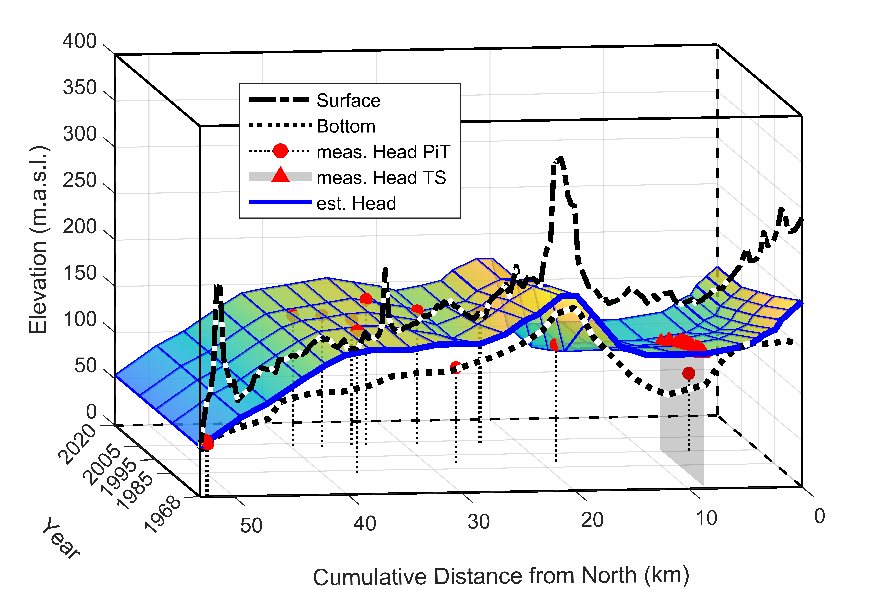
\includegraphics{./img/Fig-EasternBoundary.pdf}
    \caption{The adjusted Dirichlet boundary condition for the eastern boundary. The for 1968 estimated initial head (thick blue line) along with the bottom- (thick black dotted) and surface- (thick black dashed) elevations are shown at the starting year 1968. Measured heads are shown in in red as circles for single point-in-time (PiT) measurements and as triangles for time series (TS) measurements. The grid (blue) spanning the temporal evolution of heads shows the linear interpolation in between the 29 locations and the five specified years. For better perceptablility the surface marking the head stages in between these points is coloured according to head values.}
    \label{Fig-EastB}
\end{figure}

\subsection{Southern Boundary}

The southern boundary is defined by the Massa River. 
Due to both the temporal and spatial variability of the flow regimes along the river, changing influent and effluent conditions of the aquifer occur along this boundary. 
To account for this, \cite{Horn.2021} implemented this boundary as Chauchy boundary condition into GMS. 
Hence it is characterised through three parameters: the bottom elevation of the river channel, the head stage and the riverbed conductance. 
The bottom elevation is defined using the DEM.

The head stages are estimated by an assumed linear relation between the discharge rate measured at the YBT dam and the assumed average water level in the river. 
These discharge rates are extracted from data of daily water balances in the YBT reservoir aggregated to yearly data. 
As these measurements were taken only from 1974 onwards, once the dam became fully operational two different time periods need to be distinguished: before and after 1974. 
For the prior time period from 1968 to 1974 head stages are estimated from annual rainfalls.

The conductance $C$ $\left( \textrm{m} \, \textrm{s}^{-1} \right)$ is estimated as conductance per unit length by

\begin{equation}
    C = \frac{k}{t} w
\end{equation}

where $k$ $\left( \textrm{m} \, \textrm{s}^{-1} \right)$ is the hydraulic conductivity of the riverbed, $t$ $\left( \textrm{m} \right)$ the riverbed thickness and $w$ $\left( \textrm{m}\right)$ the width of the river \parencite{Aquaveo.2019}. 
For the hydraulic conductivity values lower than those of the underlying lithological unit are assumed, as sedimentation may lead to clogging processes.

As described in Section \ref{Sec-SouMaHydrology}, the Massa River can be divided into two different parts \parencite{Horn.2021}: an upstream part ranging from the YBT dam to the village of Ifentar, and a downstream part from Ifentar to the Atlantic Ocean. 
Therefore, on these two sections different assumptions define the applied parameters of river width and riverbed thickness. 
Higher flow velocities in the narrow upstream part lead to higher erosion and lower sedimentation in the river bed and thus a thinner riverbed is assumed. 
In the wider downstream part on the other hand less erosion and higher sedimentation occurs, leading to a thicker riverbed.

\subsection{Western Boundary}

The western boundary is defined as a Dirichlet constant head boundary. 
Its shape is defined by the coast of the Chtouka plain along the Atlantic Ocean. 
Head stages at this boundary are assumed to be at a constant sea level of $0 \, \textrm{m.a.s.l.}$ over the whole modelling period.

%%%%%%%%%%%%%%%%%%%%%%%%%%%%%%%%%%%%%%%%%%%%%%%%%%%%%%%%%%%%%%%%%%

\section{Geological Model}
\label{Sec-GeolModel}

In a previous work, \cite{Horn.2021} built a geological model of the Chtouka aquifer (Figure \ref{Fig-GeolMod}) on the basis of lithological drilling data from 100 boreholes, geophysical measurements and a geological map of the region. 
This model is used in this study and shown in Figure \ref{Fig-GeolMod}. 
In the following, its main characteristics will be summarised. 
For more detailed information refer to the cited study.

Over the modelling area, five different lithological units, each assumed as homogeneous over its spatial extent, were identified. 
These units are:

\begin{itemize}
    \item calcareous marl,
    \item gravel,
    \item sand,
    \item schist and
    \item silty sand.
\end{itemize}

Of these, calcareous marl, sand and schist form the group of main units with large spatial extents. 

Schist is considered to be the oldest stratigraphical unit. 
It outcrops in the eastern part of the aquifer and is covered by sediments towards the west. 
Above the schist lies in most regions a layer of calcareous marl with a mean thickness of $100 \, \textrm{m}$. 
Although showing in reality local variations between more sandy and more clayey areas, it is over-all assumed as one lithological unit. 
Apart from an area in the south where this lithological unit outcrops, calcareous marl is covered by one of the three remaining strata. 
Predominantly the overlying layer is sand, which also forms the top of the aquifer in most areas. 
While reaching its estimated maximum thickness of $150 \, \textrm{m}$ along the coast, the layer thins towards the eastern part. 
The north east of the model is characterised by alluvial fans of varying compositions of clay, sand and gravel in both horizontal and vertical direction. 
This area is modeled by the two lithological units silty sand and gravel. 
Each geological unit is defined by its specific material properties, which are the hydraulic conductivities $K_h$ in horizontal and $K_v$ in vertical direction (both $\left( \textrm{m} \, \textrm{s}^{-1} \right)$) as well as the corresponding horizontal and vertical anisotropies $\left( - \right)$, the porosity $\phi$ $\left( - \right)$, the specific yield $S_y$ $\left( - \right)$ and specific storage $S_s$ $\left( \textrm{m}^{-1} \right)$.

The top of the aquifer corresponds to the surface and is defined by the DEM of \cite{NASA.SRTM1Arc}, which has a $30 \, \textrm{m} \times 30 \, \textrm{m}$ resolution. 
The bottom boundary of the aquifer is defined by \cite{Horn.2021} depending on the local stratification of the lithological units. 
As a basis, unweathered schist is generally assumed to be a towards the bottom confining aquitard. 
However, schist may become a water bearing stratum due to weathering. 
Following \cite{McFadden.2005} this weathering is considered to reach at most $50 \, \textrm{m}$ into the unit. 
This maximum depth may occur only in regions where the schist crops out, as this is the case in the eastern parts of the model area. 
Where the schist is overlain by other strata, the weathered depth should accordingly be reduced (Note: This however is not directly stated in \cite{Horn.2021}, but follows from the fact that in the model schist also appears in regions where it is not the top layer). 
This leads to a minimum depth of the aquifer of $50 \, \textrm{m}$ in relation to the local surface elevation in all regions. 
In the central area, thicknesses of the aquifer are estimated by the depths of the locally deepest drilled boreholes. 
In the northern part of the Chtouka aquifer, data from measuring campaigns of vertical electrical soundings in the period 1947 to 2008 in the Souss Massa Basin are used to define the bottom of the aquifer. 
For the coastal areas, transient electromagnetics measurements (\textcite{Kalberkamp.2021}, \textcite{Terratec.2020}) from a campaign within the framework of the CREM project are used.

\begin{figure}[h]
    \centering
    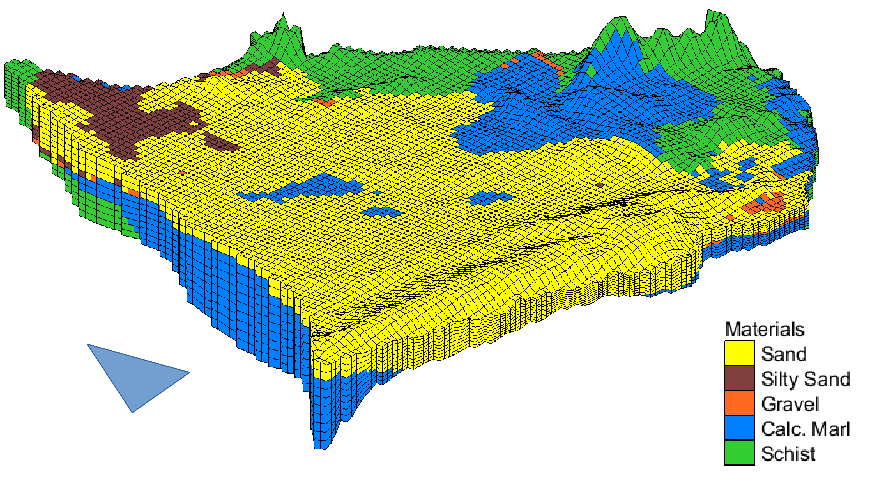
\includegraphics{./img/Fig-GeoMod.pdf}
    \caption{The already geological model of the Chtouka aquifer, as defined by \cite{Horn.2021}. The $xy$-plane is oriented along the four cardinal directions with the positive $x$-direction pointing to the north (arrow). In the $xy$-plane cell edges have a length of $500 \, \textrm{m}$. For presentation purposes, a $z$-magnification with a factor of 10 is applied.}
    \label{Fig-GeolMod}
\end{figure}

%%%%%%%%%%%%%%%%%%%%%%%%%%%%%%%%%%%%%%%%%%%%%%%%%%%%%%%%%%%%%%%%%%

\section{Recharge from Precipitation}
\label{Sec-PrecRech}

Precipitation data were compiled by \cite{Horn.2021} and will be briefly described in the following. 
For more information, refer to the cited study.
    
For estimations of the local precipitation, datasets from meteorological stations in Agadir, Ait Melloul, Ait Amira, Biougra and at the YBT dam were available. 
Based on these data three zones are identified, which account for the spatial variations of precipitations due to regional differences in altitude and climate. 
These zones are shown in Figure \ref{Map-BCPzPrec}.
    
    
The northwestern zone has the highest average annual precipitation of \linebreak $220 \, \textrm{mm} \, \textrm{a}^{-1}$ over the modelling period (1968-2020). 
The central zone, which incorporates the largest area of the model region, and the southeastern zone are characterised by a significantly lower annual precipitation of $190 \, \textrm{mm} \, \textrm{a}^{-1}$ respectively $160 \, \textrm{mm} \, \textrm{a}^{-1}$ over the modelling period.

The infiltration rates of the precipitation are estimated basing on the top-most lithological unit and expected evaporation from the ground. 
Therefrom infiltration rates of $6 \, \%$ of the precipitation follow for the northern and central areas and $5 \, \%$ for the southern area \parencite{Resing.2008}. 
The derived annual time series of recharge from precipitation are shown for the three areas in Figure \ref{Fig-RechPrec}.

\begin{figure}[h]
    \centering
    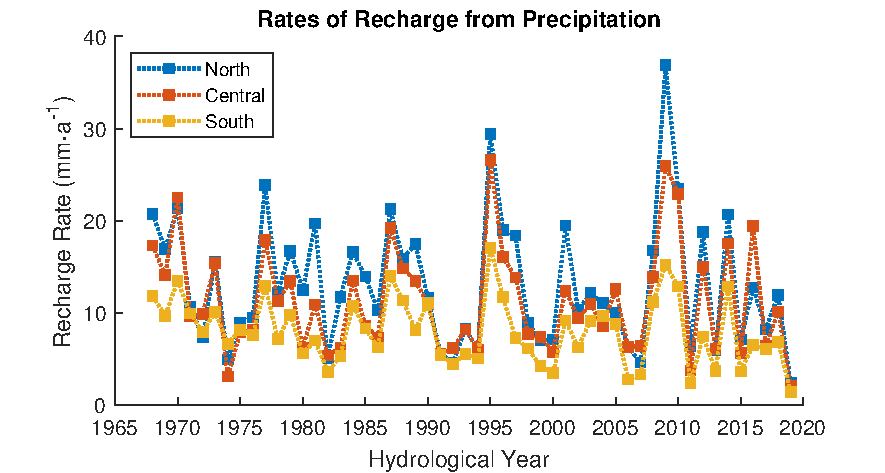
\includegraphics{./img/Fig-PrecRecharge.pdf}
    \caption{Time series of annual groundwater recharge in the three different zones (Figure \ref{Map-BCPzPrec}) as identified by \cite{Horn.2021}.}
    \label{Fig-RechPrec}
\end{figure}

%%%%%%%%%%%%%%%%%%%%%%%%%%%%%%%%%%%%%%%%%%%%%%%%%%%%%%%%%%%%%%%%%%

\section{Groundwater Wells}
\label{Sec-GWWells}

Groundwater extraction through wells has been examined in various studies by the ABHSM. 
Thus, data is available from different databases. 
This data has been previously analysed by the project team and processed to fit the modelling needs. 
In the following, the main features are summarised. 
For detailed information refer to the technical notes in Appendices A and B in \cite{Horn.2021}. 
Each well is characterised by a name, its location in the $xy$-plane and its top elevation, the depth to top of the screen and the screen length as well as by a time series of estimated or measured flow rates. 
All wells can be distinguished into two classes. 
The first class encompasses manually dug wells, the second drilled and reconaissance wells. 
This classification has been used to interpolate missing data concerning the vertical screen locations and screen lengths of some wells. 
Furthermore, the wells can be additionally classified through the utilisation of the extracted water, which is either for drinking and domestic purposes or for irrigation. 
Based on the end user, pumping rates have been estimated for wells with missing data.

\subsection{Drinking Wells}

A total of 380 wells are considered as drinking wells in the study area. 
These are depicted in Figure \ref{Map-PumpWells}(a). 
Data on extracted water volumes are available for the time periods 1969-2001 from one single source and 2001-2020 from several sources. 
Based on these datasets pumping volumes and therewith pumping rates are estimated for the whole period from 1969 to 2020. 
Information on commissioning of new wells is only available until 2003. 
After 2003, the further commissioning of wells is assumed as being coupled to the population growth and is assigned a yearly growth rate of $0.7 \, \%$, thus slowly increasing the extracted water volume.

\subsection{Irrigation Wells}

Data regarding the irrigation wells is available from two surveys carried out in 2003 and 2015. 
In the study from 2003, a total of 2448 wells are recorded and in 2015 a number of 3050 wells. 
Due to significant differences in either location (the vast majority) or in well characteristics (for wells with similar coordinates) both sets of wells are considered as disjunct. 
Therewith a total of 5498 irrigation wells is considered in this study (Figure \ref{Map-PumpWells} (b)). 
Data from the studies are based on personal records or memorizations from farmers and estimates for each well or each farm made during the surveys.

\begin{figure}[h]
    \centering
    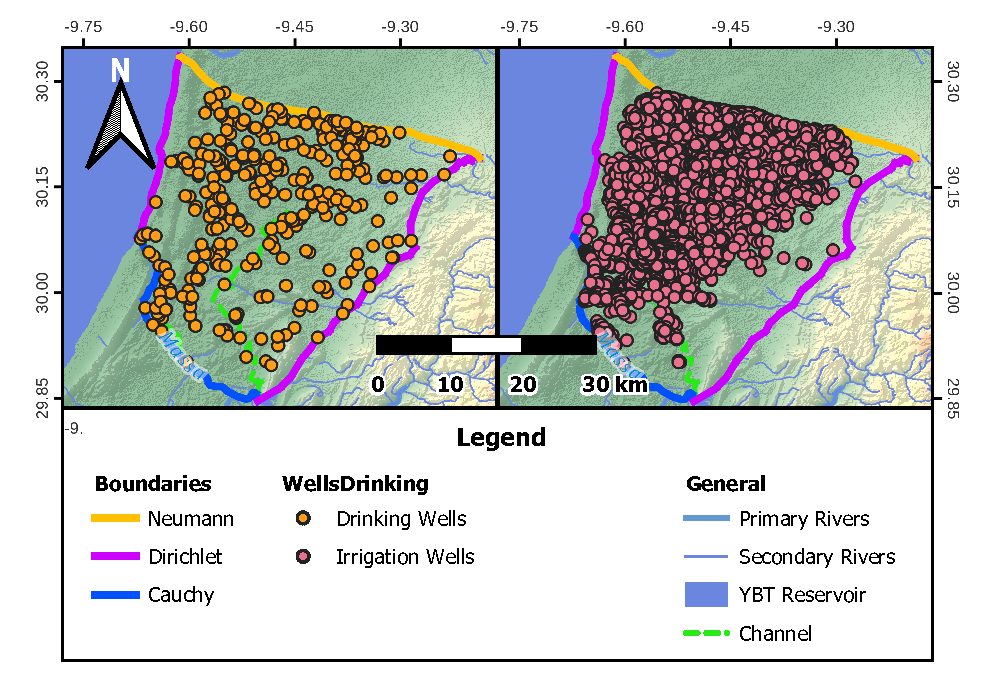
\includegraphics{./img/Map_IrrDri.pdf}
    \caption{Spatial distribution of the in this study considered 5498 irrigation wells (left) and 380 drinking wells (right).}
    \label{Map-PumpWells}
\end{figure}

%%%%%%%%%%%%%%%%%%%%%%%%%%%%%%%%%%%%%%%%%%%%%%%%%%%%%%%%%%%%%%%%%%

\section{Irrigation Returns}
\label{Sec-IrrRech}

As described in Section \ref{Sec-SouMaStructure}, the Chtouka plain is extensively used for agricultural activities. 
As stated introductorily to this section, a certain portion of the applied irrigation water re-infiltrates into the aquifer and leads to groundwater recharge. 
To account for this recharge, both the spatial extents and the infiltration rates of the applied water are estimated as described in this section.

It is assumed that the Tassila perimeter exsisted for several hundred of years in its current extents. 
The public perimeter mainly exists since the commissioning of the YBT dam. 
Therefore, the extents of both perimeters are assumed as constant. 
An analysis of satellite pictures from different years shows a significant change over time for the private perimeter. 
To account for this evolution, the perimeter's extents are estimated for six consecutive periods (1968-1973, 1974-1979, 1980-1989, 1990-1999, 2000-2009 and 2010-2020). 

Within the three perimeters the three different irrigation techniques flooding, sprinkler and drip irrigation are used. 
Inside each of the three perimeters, a homogeneous distribution of the applied techniques is assumed. 
Over time, the frequency ratios of the different methods vary as previous studies show (\cite{Resing.2003}, \cite{Anzar.2016}). 
Based on these studies the temporal evolution of the frequency ratios is estimated for each of the three perimeters. 
Infiltration rates are finally calculated depending on these distributions.

%%%%%%%%%%%%%%%%%%%%%%%%%%%%%%%%%%%%%%%%%%%%%%%%%%%%%%%%%%%%%%%%%%

\section{Observations}
\label{Sec-Piezometers}

Observational data of head measurements are available from 27 piezometers that are scattered over the study area (Figure \ref{Map-BCPzPrec}). 
These observations cover different time periods within 1968-2020.

At four locations a respective pair of piezometers is available that is covering successive time periods. 
The second ones were built as due to the local drawdown of the groundwater table the originally installed piezometers fell dry. 
From these piezometers, for each pair a combined, longer time series can be generated. 
Therewith, observations are available for 23 distinct locations.

Furthermore, the observed head data is calculated from two measurements: A one-time measurement of the $z$-location to level the top of the piezometer, and a second, continuous measurement of depth from the surface to the watertable. 
Thus, piezometers can be divided into two main groups, based on the determination of $z$: levelling and topography map reading. 
For levelled piezometers, an error of $1 \, \textrm{m}$ is assigned. 
For non-levelled piezometers, this error is $10 \, \textrm{m}$.

%%%%%%%%%%%%%%%%%%%%%%%%%%%%%%%%%%%%%%%%%%%%%%%%%%%%%%%%%%%%%%%%%%
%%%%%%%%%%%%%%%%%%%%%%%%%%%%%%%%%%%%%%%%%%%%%%%%%%%%%%%%%%%%%%%%%%
%%%%%%%%%%%%%%%%%%%%%%%%%%%%%%%%%%%%%%%%%%%%%%%%%%%%%%%%%%%%%%%%%%

\chapter{Implementation of the Model}
\label{Chap-ImplMod}

%%%%%%%%%%%%%%%%%%%%%%%%%%%%%%%%%%%%%%%%%%%%%%%%%%%%%%%%%%%%%%%%%%

\section{Implementation of the Model}

\subsection{Modelling Software: GMS}
\label{Sec-GMS}

In this study the Groundwater Modeling System (GMS) software by Aquaveo, LLC. is used as modelling environment. 
It is a common software applied in the field of hydraulic, hydrologic and groundwater modelling and is used by many federal and local governmental agencies around the world \parencite{Aquaveo.2021}.

Regarding the fundamental flow calculations GMS bases on the modular finite-difference flow model MODFLOW \parencite{McDonald.1988}, which is available in various versions. 
To simulate seawater intrusion, the three-dimensional multi-species solute transport model MT3DMS \parencite{Zheng.1999} and the variable-density groundwater flow model SEAWAT \parencite{Langevin.2009} will be applied in future studies to the here examined model. 
As SEAWAT bases on MODFLOW-2000 \parencite{Harbaugh.2000}, in this study this particular MODFLOW version is used.

MODFLOW itself is divided into a series of processes and packages. 
While major tasks are organised as processes, more specific tasks are executed by packages leading to the eponymous modularisation. 
Therefore, each optional package provides a different functionality. 
To utilise these particular functionalities, the corresponding packages need to be activated for the single elements of a GMS model.

In GMS numerical groundwater models are generated either by direct manipulations of a defined three-dimensional grid or by a conceptual modelling approach, as it is applied in this study. 
For this latter approach GMS utilises common GIS-objects such as points, arcs and polygons which are defined as distinct features on different layers. 
Each layer represents one homogeneous class of objects - one of the above mentioned feature types - which correspond to one specific term of the groundwater flow equation (Section \ref{Sec-ModEq}).

%%%%%%%%%%%%%%%%%%%%%%%%%%%%%%%%%%%%%%%%%%%%%%%%%%%%%%%%%%%%%%%%%%

\subsection{Model Equations}
\label{Sec-ModEq}

As a basis for future work, in the scope of this study the temporal evolution of a constant-density flow in the Chtouka aquifer is to be considered. 
The assumption of constant density implies two simplifications of the real world system: First the incompressibility of the flowing medium water, second the neglect of saltwater intrusion. 
Therewith the groundwater flow in the system that is schematically depicted in Chapter \ref{Chap-ConcMod} is described by the groundwater flow equation \eqref{Eq-GWFlow},

\begin{equation}
    S_s \frac{\partial h}{\partial t} \; \; = \; \; \frac{\partial}{\partial x} \left(K_{xx} \frac{\partial h}{\partial x} \right) + \frac{\partial}{\partial y} \left(K_{yy} \frac{\partial h}{\partial y} \right) + \frac{\partial}{\partial z} \left(K_{zz} \frac{\partial h}{\partial z} \right) + \dot{M}_{ss,i}
\end{equation}

where $K_{xx}$, $K_{yy}$ and $K_{zz}$ denote the hydraulic conductivities in $\left( \textrm{m} \, \textrm{s}^{-1} \right)$ along the $x$-, $y$- and $z$-axis respectively, $h$ the potentiometric head in $\left( \textrm{m} \right)$, $S_s$ the specific storage of the porous medium $\left( \textrm{m}^{-1} \right)$ and $t$ the time $\left( \textrm{s} \right)$.

$\dot{M}_{ss,i}$ denotes the different source- and sink-terms $i$ as volumetric flux per unit volume $\left( \textrm{s}^{-1} \right)$. 
These are following the conceptual model here the recharge from precipitation, the withdrawal from both drinking and irrigation wells and the irrigation returns. 
Negative values of $M_{ss,i}$ imply flow out of the system and positive values flow into the system.

As explained in Section \ref{Sec-GWFlowEq} only the diagonal elements $K_{ii}$ of the hydraulic conductivity tensor are here considered. 
In the deviation of the equation this is possible due to the arbitrary choice of orientation of the coordinate system in the single control volumes parallel to the major axes of the hydraulic conductivity \parencite{Harbaugh.2000}. 
However it may be noted that in MODFLOW-2000 only a global coordinate system is considered. 
As stated in Section \ref{Sec-Discretisation} this coordinate system is oriented along the cardinal directions.

%%%%%%%%%%%%%%%%%%%%%%%%%%%%%%%%%%%%%%%%%%%%%%%%%%%%%%%%%%%%%%%%%%

\subsection{Implementation of the Conceptual Model in GMS}
\label{Sec-ImplToGMS}

The in this study used geological model was implemented by \textcite{Horn.2021} in GMS first as a triangulated irregular network (TIN). 
It was then discretised as described in Section \ref{Sec-Discretisation}. 
The material properties of the geological units that are relevant for this study are the hydraulic conductivities $K$ and specific storage $S_s$, as can be seen from the groundwater flow equation \eqref{Eq-GWFlow}. 
In this study the hydraulic conductivities are assumed to be horizontally isotropic, $K_{xx} = K_{yy}$, and in vertical direction to have an anisotropy with a factor of 10, $K_{xx} = 10 \cdot K_{zz}$. 
As the geological model represents a simplification of the aquifer, exact values of the named parameters need to be estimated basing on the model's behaviour. 
This is described in Section \ref{Sec-SAnaCal}.

The other layers of the in Chapter \ref{Chap-ConcMod} described conceptual model are imported as distinct layers into GMS. 
The different features corresponding to each layer are represented by one of the common GIS-objects, as specified in Table \ref{Tab-GMSLayersOV}. 
The different MODFLOW packages applied to each layer are listed here as well. 
As GMS can process only non-overlapping polygons in one layer, the over time varying private irrigation perimeters are defined on several layers. 
Therefore each identified period of constant extents (e.g. 1968-1973, see Section \ref{Sec-IrrRech}) is implemented in a single layer, leading to a total of six layers for the private irrigation perimeter. 
As the public and Tassila perimeters do not overlap, these are assigned to one single, shared layer.

\begin{table}[h]
    \centering
    \caption{Overview of the in GMS implemented layers. Each layer is comprised of features of the specified object class and utilises the listed MODFLOW packages. $^{(*)}$: The time-dependent areas of the private perimeter are divided by corresponding periods into six layers (Section \ref{Sec-GMS}).}
    \label{Tab-GMSLayersOV}
    \begin{tabular}{ccc}
        Layer                                   & GIS-feature type & utilised packages \\ \hline
        Boundary East                           & arc              & LPF, CHD1         \\
        Boundary South                          & arc              & LPF, RIV1         \\
        Boundary West                           & arc              & LPF, CHD1         \\
        Precipitation Areas                     & polygon          & RCH1              \\
        Drinking Wells                          & point            & WEL1              \\
        Irrigation Wells                        & point            & WEL1              \\
        Irrigation Returns Private (6x)$^{(*)}$ & polygon          & RCH1              \\
        Irrigation Returns Public+Tassila       & polygon          & RCH1              \\
        Piezometers                             & point            & Trans. Head      
        \end{tabular}
\end{table}

%%%%%%%%%%%%%%%%%%%%%%%%%%%%%%%%%%%%%%%%%%%%%%%%%%%%%%%%%%%%%%%%%%

\subsection{Discretisation}
\label{Sec-Discretisation}

The groundwater flow equation \eqref{Eq-GWFlow} is a non-linear, inhomogeneous partial differential equation. 
Therefore it cannot trivially be solved analytically for the described system. 
Within the framework of GMS the equation is therefore solved numerically. 
A three-dimensional cartesian grid is generated and Equation \eqref{Eq-GWFlow} is solved on this grid for defined time steps using the finite difference method. 
For further details on the solution method refer to \textcite{Harbaugh.2000}.

\subsubsection{Spatial Discretisation}

In this study the by \cite{Horn.2021} derived three-dimensional discretised geological model is used. 
It bases on an implementation of the original geological model as from which the three dimensional grid was generated using the grid overlay approach in MODFLOW-2000.

In horizontal direction the resulting grid has a quadratic cell size of $500 \, \textrm{m} \, \times 500 \, \textrm{m}$ with cell edges oriented in the four cardinal directions. 
Positive $x$-direction points to the east, positive $y$-direction to the north (Figure \ref{Fig-GeolMod}). 
In vertical direction, the model is set to a thickness of 10 equally spaced layers with therefore in $x$- and $y$-direction locally varying depths. 
Positive $z$-direction points upwards. 
The minimum layer thickness is set to $2.5 \, \textrm{m}$. 
The top- and bottom-most cell faces are defined as variably shaped surfaces, depending on the DEM and the bottom of the solids. 
The shapes of the inter-cellular faces are linearily interpolated between the outer two. 
To each cell the lithological unit locally incorporating the largest volume is assigned, defining the cell's material properties.

\subsubsection{Temporal Discretisation}

Regarding the temporal discretisation, MODFLOW 2000 utilises a division into stress periods and time steps. 
Stress periods are generally defined in GMS as periods of constant transient stresses (e.g. pumping rates, precipitation). 
Each stress period can have a particular length and is further sub-divided into a number of equally long time steps.

For this model stress periods are defined as the single hydrological years, which start on 1st of September at ${00\!:\!00\!:\!00}$ of one year and end on 31st of August of the subsequent year at ${23\!:\!59\!:\!59}$. 
They therewith show a variable length due to leap years. 
The number of time steps is set to two per stress period. 
The correctness of this approach was successfully tested through comparison of simulations with otherwise constant parameters, showing equality.

%%%%%%%%%%%%%%%%%%%%%%%%%%%%%%%%%%%%%%%%%%%%%%%%%%%%%%%%%%%%%%%%%%

%%%%%%%%%%%%%%%%%%%%%%%%%%%%%%%%%%%%%%%%%%%%%%%%%%%%%%%%%%%%%%%%%%

\section{Methodology of Sensitivity Analysis and Calibration}
\label{Sec-SAnaCal}

The true behaviour $T$ of a system can be either measured, through which an experimental value $E$ is obtained. 
Or it can be modeled, which yields a modelling value $M$. 
In either case, the results obtained deviate from reality due to measuring errors $\delta_E$ or modelling errors $\delta_{SM}$ \parencite{Stern.2001},

\begin{align}
    T & =  E - \delta_E \label{Eq-ValueEx} \\
    T & =  M - \delta_{SM} \label{Eq-ValueModel}
\end{align}

Although models represent a simplified version of reality, they are often described by complex mathematical equations that cannot be solved analytically. 
Therefore the exact modelling value $M$ is numerically approximated by a simulation value $S$. 
Likewise, this value underlies a numerical error $\delta_{SN}$ \parencite{Stern.2001},

\begin{equation}
    \label{Eq-ValueSim}
    M = S - \delta_{SN}
\end{equation}

The simulation result can be expressed as function $f$ of system inputs (the key variables) $\bm{X}$ and parameter combinations $\bm{\theta}$ \parencite{Naeini.2019},

\begin{equation}
    \label{Eq-FunSim}
    S = f(\bm{X},\bm{\theta})
\end{equation}

In this study each specific combination $\bm{\theta} = ( \theta_1,\dots,\theta_N)$ of values $\theta_i$ of the $N$ different parameters $i$ is called a parameter set. 
All possible parameter sets constitute the parameter space $\Theta$.

The adequacy of a model for a specific purpose can be assessed through its capability to describe the behaviour of the real system. 
Thus with Equations \eqref{Eq-ValueModel}, \eqref{Eq-ValueSim} and \eqref{Eq-FunSim} follows:

\begin{equation}
    \label{Eq-CompSimTruth}
    T = f(\bm{X},\bm{\theta}) - (\delta_{SM} + \delta_{SN})
\end{equation}

To achieve a close fit of the model to the reality, it is necessary to minimise the numerical and modelling errors. 
The prior can be decreased among others through the choice of an adequate discretisation and solution scheme as well as through the refinement of the discretisation. 
The latter depends on both the modelling function $f$ itself and the choice of a suitable parameter set $\bm{\theta}$. 
$f$ is defined through the modelling equations whose exact formulation depends on the conceptual model. 
Therefore after assembling a model to a state as far as described for the here applied model, a further reduction of the simulation error is only possible through an adjustment of the model parameter values $\bm{\theta}$.

A model's response significantly depends on these parameters. 
An example is shown in Figure \ref{Fig-ParamSpaceEx}. 
Depending on the choice of the specific parameter set, the modelling error varies. 
This variation is generally non-linear and can show a great deal of interaction between the different parameters \parencite{Duan.1993}. 
Thus within the parameter space $\Theta$ not only one global optimum may exist for which the modelling error reaches its global minimum ($\bm{\theta}_{go}$ corresponding to a point within the green area in Figure \ref{Fig-ParamSpaceEx}). 
But there also may be several other local optima at which the modelling error becomes locally minimal. 
In Figure \ref{Fig-ParamSpaceEx} these are within the closed yellow and orange areas in the top-left, of which one is exemplarily marked corresponding to $\bm{\theta}_{lo}$.

\begin{figure}[h]
    \centering
    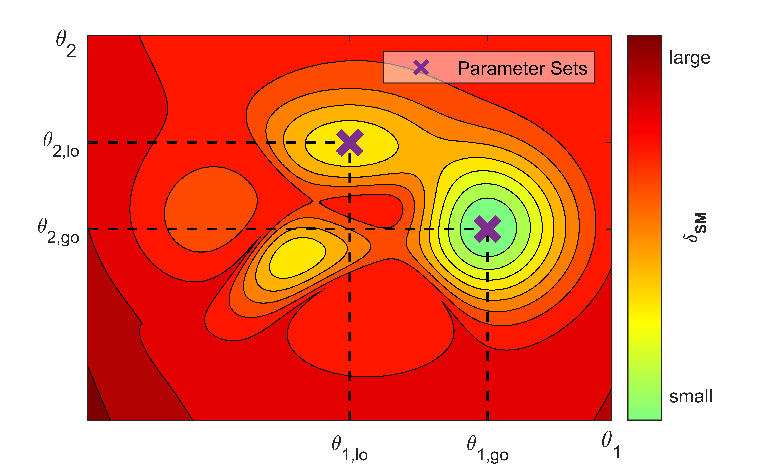
\includegraphics{./img/Fig-ParamSpaceEx.pdf}
    \caption{Example of a two dimensional continuous parameter space $\Theta$ with elements $\bm{\theta} = \left(\theta_{1,i}, \theta_{2,j}\right)$. Each of these parameter sets corresponds to an absolute modelling error $\delta_{SM}$ marked by the colour scale. In this example, the parameter set $\bm{\theta}_{lo}$ corresponds to a local minimum of the modelling error $\delta_{SM}$. The global optimum of $\delta_{SM}$ is obtained by the parameter set $\bm{\theta}_{go}$.}
    \label{Fig-ParamSpaceEx}
\end{figure}

The process of finding the parameter set corresponding to the global minimum of $\delta_{SM}$ is called calibration. 
The procedure used in this study is described in Section \ref{Sec-SubMethCal}. 

As the function $f(\bm{X},\bm{\theta})$ is often unknown, calibration needs to be conducted by simple trial-and-error. 
Therefore it is computationally expensive and if carried out manually also very time-consuming. 
However, not all model parameters impact the model results equally extensive \parencite{Duan.1993}. 
Therefore, the number of parameters considered in calibration of a model can preliminarily be reduced to only those parameters with significant impact. 
To identify these different impacts, the behaviour of the model to changes in single parameters is examined in a sensitivity analysis prior to the calibration. 
The procedure of the sensitivity analysis that this study follows is described in Section \ref{Sec-SubMethSAna}. 

Crucial to the success of both sensitivity analysis and calibration is the meaningful measurement of the modelling error $\delta_{SM}$. 
Several different measures exist that have different characteristics. 
Section \ref{Sec-SubMethErrAss} describes the methodology followed in this work.

Prior to sensitivity analysis and calibration however, the examined parameters need to be identified. 
In this study, not all model parameters are taken into account. 
Those examined in the sensitivity analysis are described in the following Section \ref{Sec-SubMethParams}.

%%%%%%%%%%%%%%%%%%%%%%%%%%%%%%%%%%%%%%%%%%%%%%%%%%%%%%%%%%%%%%%%%%

\subsection{Examined Parameters}
\label{Sec-SubMethParams}

In this study, three groups of parameters are identified for which the model is to be calibrated. 
Two of these directly follow from the groundwater flow equation \eqref{Eq-GWFlow}: the hydraulic conductivities $K_{ii}$ and the specific storage $S_s$. 
For the third one it is acknowledged that the estimations of the pumping rates underly a large uncertainty. 
Therefore the associated sink-term $\dot{M}_{ss,irr}$ is provided with a scaling factor $\theta_{Q,irr}$.

Both the hydraulic conductivities and the specific storages are material properties and characterise the geological model for the flow model. 
Therefore, both have specific values for each of the five lithological units into which the model is divided. 
Although each of the parameters therewith corresponds to a defined unit, exact values are unknown. 
This is due to the coarse classification into five lithological units of the possibly more heterogeneous geology of the aquifer. 
Likewise, characterisations in literature differ.

A within the project framework conducted literature research identified for hydraulic conductivities a range of values over several orders for each material. 
The corresponding minimum and maximum values are listed in Table \ref{Tab-MatPropsRange}. 
Therewith no direct specification between the hydraulic conductivities in $x$-, $y$- and $z$-direction are possible. 
To reduce the dimensions of the parameter space, certain assumptions are made. 
First, as the flow directions in the $xy$-plane vary in space while no location-dependent variation of $K_{xx}$ and $K_{yy}$ is possible within the model framework, a horizontal isotropy is assumed,

\begin{equation}
    K_h \; = \; K_{xx} \; = \; K_{yy}
\end{equation}

\noindent where $K_h$ is the horizontal hydraulic conductivity. 
Second, a constant anisotropy between horizontal and vertical hydraulic conductivity is assumed with a proportionality factor of 10,

\begin{equation}
    K_h \; = \; 10 \, K_v \; = \; 10 \, K_{zz}
\end{equation}

\noindent with the vertical hydraulic conductivity $K_v$. 
In the following the hydraulic conductivities will be expressed in terms of the horizontal hydraulic conductivities $K_{h}^{(i)}$ of the materials $i$.

In the same, prior to this study conducted literature research it was found that few values for the specific storage are available in literature. 
Therefore, more data concerning the specific yield and the effective porosity of probes is given. 
Thus, the values for the specific storage are approximated with Equation \eqref{Eq-SsSy} through the specific yield $S_y$ and the aquifer thickness $b$. 
Values for the specific yield can either be measured directly or approximated as equalling the effective porosity of a probe. 
The identified range of values for these two quantities are shown in Table \ref{Tab-MatPropsRange}. 
The aquifer thicknesses $b$ refer to average thicknesses of the respective lithological units. 
However, these thicknesses are not constant but vary significantly in space. 
To account for this the geological model is examined statistically. 
From this analysis ranges of the material thicknesses are estimated. 
The corresponding limits are defined by the $20 \, \%$- and $80 \, \%$-Quantiles (Table \ref{Tab-MatPropsRange}). 
From these estimations of $S_y$ and $b$ the ranges of values for the material-specific specific storages are calculated as described. 
The results are shown in Table \ref{Tab-MatPropsRange}. 
In the following the specific storages will be expressed as $S_{s}^{(i)}$ of the materials $i$. 

\begin{table}[h]
    \label{Tab-MatPropsRange}
    \caption{Overview of the value ranges of the parameters horizontal hydraulic conductivity $K_h$ and specific storage $S_s$ for all materials. Furthermore the value ranges of specific yield $S_y$ and material thickness $b$ are listed that were used to calculate the specific storages.}
    \begin{tabular}{clcclcclcclcc}
        Material   & $\; \;$ & \multicolumn{2}{c}{$K_h$ $(\textrm{m} \, \textrm{s}^{-1})$} & $\; \;$ & \multicolumn{2}{c}{$S_y$ $(-)$} & $\; \;$ & \multicolumn{2}{c}{$b$ $(\textrm{m})$} & $\; \;$ & \multicolumn{2}{c}{$S_s$ $(\textrm{m}^{-1})$} \\ \hline
        Calc. Marl &         & $1 \cdot 10^{-6}$            & $1 \cdot 10^{-4}$            &         & 23             & 38             &         & 21                & 109                &         & $2 \cdot 10^{-3}$     & $2 \cdot 10^{-2}$     \\
        Gravel     &         & $1 \cdot 10^{-7}$            & $9 \cdot 10^{-5}$            &         & 2              & 10             &         & 20                & 85                 &         & $2 \cdot 10^{-4}$     & $4 \cdot 10^{-3}$     \\
        Sand       &         & $8 \cdot 10^{-5}$            & $1 \cdot 10^{-2}$            &         & 17             & 24             &         & 13                & 54                 &         & $3 \cdot 10^{-3}$     & $2 \cdot 10^{-2}$     \\
        Silty Sand &         & $1 \cdot 10^{-7}$            & $1 \cdot 10^{-3}$            &         & 10             & 40             &         & 32                & 350                &         & $3 \cdot 10^{-4}$     & $1 \cdot 10^{-2}$     \\
        Gravel     &         & $4 \cdot 10^{-7}$            & $5 \cdot 10^{-4}$            &         & 1              & 26             &         & 23                & 140                &         & $7 \cdot 10^{-5}$     & $1 \cdot 10^{-2}$    
    \end{tabular}
\end{table}

Regarding the uncertainties of the pumping rates of the irrigation wells, prior to this study an expert on plant hydrology was consulted. 
An assessment was done on how realistic the yearly withdrawn water volumes might be. 
The estimations base on the expectable evapotranspiration when taking into account the irrigated area and cultivated plant species. 
As result, an underestimation of water withdrawal volumes by a factor of 2 was deemed possible. 
Thus, the range of values for the scaling factor of the irrigation flow rate is set to an interval of 

\begin{equation}
    \theta_{Q,irr} = \left[ 0.5, 2.0 \right]
\end{equation}

In total, a parameter set $\bm{\theta}$ therewith comprises of five values of hydraulic conductivities, five values of specific storages and one value of the scaling factor $\theta_{Q,irr}$ of the irrigation flow rate. 
The parameter space is accordingly 11-dimensional.

%%%%%%%%%%%%%%%%%%%%%%%%%%%%%%%%%%%%%%%%%%%%%%%%%%%%%%%%%%%%%%%%%%

\subsection{Methodology of the Sensitivity Analysis}
\label{Sec-SubMethSAna}

For the sensitivity analysis a basic parameter set $\bm{\theta}_3$ is picked as reference. 
To examine the model's behaviour in respect to the different parameters, each parameter is varied seperately in respect to this parameter set within its defined ranges. 
The model's behaviour to changes of this single parameter within the defined parameter set is assumed as being representative also for other parameter sets. 
Therefore the underlying parameter set is chosen to represent average values of the parameters and not extreme values. 
Thus, $\bm{\theta}_3$ is defined as the geometric averages of the different parameters. 
In this study, the model's response $S$ is evaluated for five values of each parameter. 
    
The hydraulic conductivities and specific storages from Table \ref{Tab-MatPropsRange} often range over several orders. 
Therefore a logarithmic partition of the defined intervals is applied with constant proportionalities between neighbouring values. 
Accordingly, the middle value $\theta_{i,3}$ of parameter $i$ denotes the geometrical average. 
The set of the five examined values $\theta_{i,1},...,\theta_{i,5}$ is defined by

\begin{equation}
    \label{Eq-ParamValCalc}
    \bigcup_{j=1,...,n} \theta_{i,j} \; : \; \theta_{i,j} = \left( \frac{\textrm{Max}(\Theta^{(i)})}{\textrm{Min}(\Theta^{(i)})} \right) ^{\frac{j-1}{n-1}} \cdot \textrm{Min}(\Theta^{(i)})
\end{equation}

\noindent where $n$ is the number of values, thus $n=5$. 
The response $S$ of the model is measured through analysis of the dependent variable head $h$, as described in Section \ref{Sec-SubMethErrAss}.

\subsection{Methodology of the Calibration}
\label{Sec-SubMethCal}

The goal of the calibration is to identify a parameter set $\bm{\theta}$ that globally minimises the modelling error $\delta_{SM}$. 
However, as described before also local minima of $\delta_{SM}$ may exist, and therewith several major areas to which a search strategy may converge within the feasible parameter space as described by \textcite{Duan.1993}. 
Within these areas possibly numerous local optima both close to and at various distances from the best solution may be localised. 
Furthermore, the parameters can show a great deal of - possibly non-linear - interaction and compensation \parencite{Duan.1993}. 
Thus, the start of a search strategy requires a large enough number of points to identify major areas of attraction. 
Within these areas a succeeding clustering focussed on the most promising regions is recommended. 
However, the clustering should not be limited to a small area to sustain robustness of the search against local optima \parencite{Duan.1993}.

In this work, the calibration is conducted manually, including both the changing of the parameter values on each simulation run and the corresponding evaluation of the model's results. 
In the following, the algorithm used as orientation is described. 
However, deviations from the strict pattern appear. 
This is since during the original calibration process the ranges of the single parameters were adjusted, for various reasons.

As the calibration is conducted solely manually in this study, a parallel multi-dimensional clustering is not feasible. 
Therefore a sequential approach is applied, that is divided into a number of steps $k$. 
Each such step is comprised of an cycle over the different parameters. 
Within each such cycle, the parameters are optimised succeedingly with a single iteration. 
Therefore, for each iteration an interval $[\theta_{i,k,min}, \theta_{i,k,max}]$ for parameter $i$ is defined. 
On this interval, $n=5$ or $n=7$ values are calculated in analogy to Equation \eqref{Eq-ParamValCalc} by

\begin{equation}
    \label{Eq-ParamValCalcCalib}
    \bigcup_{j=1,...,n} \theta_{i,k,j} \; : \; \theta_{i,k,j} = \left( \frac{\theta_{i,k,max}}{\theta_{i,k,min}} \right) ^{\frac{j-1}{n-1}} \cdot \theta_{i,k,min}
\end{equation}

\noindent The interval boundaries $\theta_{i,k,min}$ and $\theta_{i,k,max}$ are defined as the nearest neighbours $\theta_{i,k-1,j-1}$ and $\theta_{i,k-1,j+1}$ of the optimal value $\theta_{i,k-1,j}$ from the previous step $k-1$. 
If $j=1$ or $j=n$, $Min(\Theta^{(i)})$ or $Max(\Theta^{(i)})$ is used as respective lower or upper interval limit. 
From these parameter values, the one with the smallest corresponding error $\delta_{SM}$ is chosen. 
Through this approach it is tried to avoid a too focussed clustering while maintaining a sufficient reduction of interval limits over each iteration, and thus keeping a balance between computational costs, robustness and accuracy. 
Calibration is stopped when either the simulation output shows throughout one step only small variations or the limits of the parameter space are reached.

\subsection{Error Assessment}
\label{Sec-SubMethErrAss}

Common measures for error estimation are the root mean square error ($RMSE$) and the mean absolute error ($MAE$). 
These average single errors $y_i - \hat{y}_i$ between a measurement value $y_i$ and a reference value $\hat{y}_i$ over all $n$ instances $i$ through different averaging methods. 
$RMSE$ and $MAE$ are defined by

\begin{align}
    RMSE \; & = \; \sqrt{ \sum_{i=1}^{n} \frac{(y_i - \hat{y}_i)^2}{n} } \label{Eq-RMSE}\\
    MAE \; & = \; \frac{y_i - \hat{y}_i }{n} \label{MAE}
\end{align}


\noindent The mean absolute error therewith represents the arithmetic average of the single errors $y_i-\hat{y}_i$, thus giving each error the same weight on a linear scale. 
The $RMSE$ on the other hand, as it first squares the single errors, weights larger errors higher than smaller errors.

In the previous study by \textcite{Horn.2021}, the error of the model was estimated through these two measures. 
Therefore the spatially distributed measuring points were regarded as an ensemble. 
Thus the underlying 3-dimensional continuous scale holding the spatial information could be reduced to a 1-dimensional nominal scale, with the identifier being the piezometer name. 
Therewith an average response of the model - where the aquifer is regarded as a unit - to changes in parameter values could be estimated. 
In this study however, the model is regarded in transient state. 
This introduces an additional dimension, the time. 
This dimension's scale, as it is discrete and not nominal, holds information about correlations between the values. 
Trivially, values at later times depend on values at preceding times. 
Using one of the aforementioned error measures thus leads to loss of information about these dependencies, since every point in time is regarded as an independent instance. 
This issue is illustrated in Figure \ref{Fig-RMSEvsCorr} (a): All three simulations have the same $RMSE$ in comparison to the observation time series, but their temporal evolution deviates significantly from each other. 
Simulation 1 shows no time dependent behaviour at all. 
In case of Simulation 2 the long-term trend matches that of the observation. 
However, the results underlie an offset in head. 
In case of Simulation 3 the initial offset is even larger, but diminishes until the end of the measuring period due to an underestimation of the long-term trend. 
An error analysis using the $RMSE$ could not distinguish between these different cases. 
However, depending on the application the different behaviours may be suitable in different ways. 
Therefore, the $RMSE$ and the $MAE$ - for analogue reasons - are deemed unfit for the assessment of time series data as in this study.

\begin{figure}[h]
    \centering
    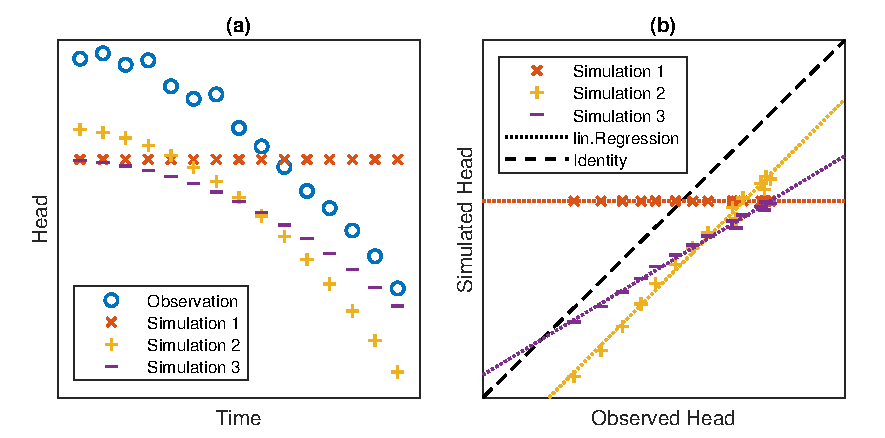
\includegraphics{./img/Fig-RMSEvsCorr.pdf}
    \caption{(a): Time series of an observation and of three simulations with different parameter sets. In comparison with the observation all three simulations have an equal $RMSE$. (b): Linear representation of the correlations between observed and simulated heads for the three simulations from (a). The respective data sets are each fitted with a linear (lin.) regression. The black dashed line marks identity between observed and simulated head.}
    \label{Fig-RMSEvsCorr}
\end{figure}

To derive a more adequate measuring method the correlation between the observed dependent variable and the simulated dependent variable are considered. 
In Figure \ref{Fig-RMSEvsCorr} this is illustrated for the here used dependent variable head $h$. 
As basis, it is assumed that a correlation between these two exists and that it can be approximated as linear relationship. 
Therewith it can be parametrised through linear regression,

\begin{equation}
    \label{Eq-ErrMethLinReg}
    S \approx p_0 + p_1 \, E
\end{equation}

\noindent with the regression coefficients $p_0$ and $p_1$. 
The therewith defined linear curves are also depicted in Figure \ref{Fig-RMSEvsCorr}.

Graphically, $p_1$ denotes the slope of the curve. 
For determination of the coefficients, least-squares fitting is applied in this study. 
Therewith, values in proximity to the limits affect the choice of $p_1$ with a higher weight, as in these regions the residuals are more sensitive to the coefficient. 
Under the assumption that short-term fluctuations of hydraulic head in an aquifer are of significantly smaller amplitude than long-term trends, this coefficient is primarily affected by the latter. 
Thus, $p_1$ can be understood as comparing the long-term trends of simulation $S$ and observation $E$ with each other. 
Values $p_1 \approx 1$ denote a similar representation of the trends from the observations by the simulation. 
Values $p_1 > 1$ or $0 < p_1 < 1$ indicate an overestimation or an underestimation of the observed trend, respectively. 
Values $p_1 < 0$ denote an under- or overestimation of the trend, but in opposite direction - e.g. while in the observed time series a drawdown of hydraulic head exists, the simulation results would give an increase in hydraulic head.


To estimate long-term trends from observational data, observations need to cover sufficiently long time periods. 
In this study, only time series covering 7 or more years are considered for estimation of $p_1$. 
Furthermore, as at four locations a respective pair of piezometers is covering seperate time periods (Section \ref{Sec-Piezometers}), their time series are merged pairwise. 
To account for the higher certainty at these locations, each piezometer is in the evaluation still considered a single independent observation point, but with the merged time series. 
This gives each of the piezometer pairs a doubled weight in respect to the other piezometers.

$p_0$ denotes the intercept of the fitted curve with the $y$-axis of the correlation plot. 
In this application it marks therewith the simulation value that would occur for an observation value $E = 0$. 
Such a value however may not be reached in the described, real system, and thus $p_0$ is a primarily mathematical quantity. 
Furthermore, $p_0$ highly depends on the interval of simulation values and empirical values that are compared. 
For intervals over large observation values of exclusively the same sign, small changes in $p_1$ result in significant changes of $p_0$. 
Also, each measuring location may have an individual observation error $\delta_E$. 
For the aforementioned issues however, this error cannot directly be incorporated into $p_0$. 
To overcome these issues, a standardisation in respect to the actual values of $S$ and $E$ is necessary. 
As in this study time series are regarded, the initial offset

\begin{equation}
    \label{Eq-ErrMethDS0-1}
    \Delta S_0 \; \; = \; \; T(t\!=\!0) - S(t\!=\!0)
\end{equation}

\noindent is chosen as representation of the true parallel shift between the truth $T$ and the simulation $S$ at time $t\!=\!0$. 
However, in this study only 8 out of 27 available observation time series date back to the here chosen initial date, the year 1968. 
To still allow the assessment of the other time series in respect to this characteristic, values are extrapolated for $T(t\!=\!0)$ in the affected cases. 
Therefore the assumption is made that the modeled trends sufficiently correlate to the observed trends. 
To obtain an expression for $T(t\!=\!0)$, Equation \eqref{Eq-ErrMethLinReg} can first be written for $t\!=\!0$ as

\begin{equation}
    \label{Eq-ErrMethDS0-2}
    S(t\!=\!0) \; \; = \; \; p_0 + p_1 \cdot E(t\!=\!0)
\end{equation}

\noindent Solving for $E(t\!=\!0)$ yields

\begin{equation*}
    \label{Eq-ErrMethDS0-3}
    E(t\!=\!0) \; \; = \; \; \frac{S(t\!=\!0) - p_0}{p_1}
\end{equation*}

Together with Equation \eqref{Eq-ValueEx}, Equation \eqref{Eq-ErrMethDS0-4} can thus be written as

\begin{equation*}
    \label{Eq-ErrMethDS0-4}
    \Delta S_0 \; \; = \; \; \frac{S(t=0) - p_0}{p_1} - \delta_E - S(t\!=\!0)
\end{equation*}

\noindent rewriting finally yields

\begin{equation}
    \label{Eq-ErrMethDS0}
    \Delta S_0 \; \; = \; \; S(t\!=\!0) \cdot \left( \frac{1}{p_1} - 1 \right) - \frac{p_0}{p_1} - \delta_E
\end{equation}

As $\Delta S_0$ depends on $1/p_1$, it may be noted that $\Delta S_0$ is only defined for values $p \neq 0$.

In real systems, numerous processes occur that influence its behaviour in different extents. 
A model does not account for all these processes. 
Furthermore measurements of dependent variables, that are also modeled underlie measuring errors $\delta_E$. 
Together, this leads to fluctuations in the measurement value $E$ that are not reproduced by a model. 
Likewise, inaccurate modelling of single processes can lead to fluctuations of the simulation value $S$ in respect to $E$ (which is strictly speaking equivalent the former and in formulation only a matter of perspective). 
Such fluctuation highly influence the accuracy of the here applied error measurement approach, as it bases on the assumption of some linear correlation between observation and simulation result. 
To which extent a model is able to reproduce the variation of the observations through simulation results, and whether it adds more fluctuation than is actually present in the observational data can be estimated by the coefficient of determination, $R^2$ \parencite{Mosteller.1977}. 
It is defined by

\begin{equation}
    \label{Eq-R2}
    R^2 \; \; = \; \; \left( \frac{ n \sum (S \cdot E) - (\sum S) (\sum E) }{ \sqrt{ [ n \sum S^2 - (\sum S)^2 ] \cdot [ n \sum E^2 - (\sum E)^2 ] } } \right)^2
\end{equation}

with $n$ denoting the number of elements of the respective time series. 
As can be seen from the definition, $R^2$ is symmetrical and can therefore be understood as how much of the variation of $E$ can be explained by $S$, and vice versa. 
Its values range between 0 and 1, with values close to 0 indicating weak linear correlation between variations, and 1 indicating high linear correlation.

%%%%%%%%%%%%%%%%%%%%%%%%%%%%%%%%%%%%%%%%%%%%%%%%%%%%%%%%%%%%%%%%%%